%%% LaTeX Template: Two column article
%%%
%%% Source: http://www.howtotex.com/
%%% Feel free to distribute this template, but please keep to referal to http://www.howtotex.com/ here.
%%% Date: February 2011

%%% Preamble
\documentclass[	DIV=calc,%
							paper=a4,%
							fontsize=12pt,%
							onecolumn]{scrartcl}	 					% KOMA-article class

\usepackage{lipsum}													% Package to create dummy text
\usepackage[brazil]{babel}										% English language/hyphenation
\usepackage[protrusion=true,expansion=true]{microtype}				% Better typography
\usepackage{amsmath,amsfonts,amsthm}					% Math packages
\usepackage[pdftex]{graphicx}									% Enable pdflatex
\usepackage[svgnames]{xcolor}									% Enabling colors by their 'svgnames'
\usepackage[hang, small,labelfont=bf,up,textfont=it,up]{caption}	% Custom captions under/above floats
\usepackage{epstopdf}												% Converts .eps to .pdf
\usepackage{subfig}													% Subfigures
\usepackage{booktabs}												% Nicer tables
\usepackage{fix-cm}													% Custom fontsizes
\usepackage[utf8]{inputenc}
\usepackage[top=2.5cm, bottom=2.5cm, left=2.5cm, right=2.5cm]{geometry}
\usepackage[ddmmyyyy]{datetime}
\addto\captionsenglish{%
	\renewcommand\tablename{Tabela}
	\renewcommand\figurename{Figura}
} 
 

 
%%% Custom sectioning (sectsty package)
\usepackage{sectsty}													% Custom sectioning (see below)
\allsectionsfont{%															% Change font of al section commands
	\usefont{OT1}{phv}{b}{n}%										% bch-b-n: CharterBT-Bold font
	}

\sectionfont{%																% Change font of \section command
	\usefont{OT1}{phv}{b}{n}%										% bch-b-n: CharterBT-Bold font
	}



%%% Headers and footers
\usepackage{fancyhdr}												% Needed to define custom headers/footers
	\pagestyle{fancy}														% Enabling the custom headers/footers
\usepackage{lastpage}	

% Header (empty)
\lhead{}
\chead{}
\rhead{}
% Footer (you may change this to your own needs)

%% ====================================
%% ====================================
%% mude o rodape  do projeto
%% ====================================
%% ====================================

\lfoot{\footnotesize \texttt{Clinica Médica XYZ} \textbullet ~Projeto de Cabeamento}


\cfoot{}
\rfoot{\footnotesize página \thepage\ de \pageref{LastPage}}	% "Page 1 of 2"
\renewcommand{\headrulewidth}{0.0pt}
\renewcommand{\footrulewidth}{0.4pt}



%%% Creating an initial of the very first character of the content
\usepackage{lettrine}
\newcommand{\initial}[1]{%
     \lettrine[lines=3,lhang=0.3,nindent=0em]{
     				\color{DarkGoldenrod}
     				{\textsf{#1}}}{}}



%%% Title, author and date metadata
\usepackage{titling}															% For custom titles

\newcommand{\HorRule}{\color{DarkGoldenrod}%			% Creating a horizontal rule
									  	\rule{\linewidth}{1pt}%
										}

\pretitle{\vspace{-30pt} \begin{flushleft} \HorRule 
				\fontsize{50}{50} \usefont{OT1}{phv}{b}{n} \color{DarkRed} \selectfont 
				}

%% ====================================
%% ====================================
%% mude o titulo  do projeto
%% ====================================
%% ====================================

\title{Clinica Médica XYZ - Projeto de Cabeamento}					% Title of your article goes here

%% ====================================



\posttitle{\par\end{flushleft}\vskip 0.5em}

\preauthor{\begin{flushleft}
					\large \lineskip 0.5em \usefont{OT1}{phv}{b}{sl} \color{DarkRed}}
\author{Lucas Rudek, Marinês Ramos}  	% Author name goes here


\postauthor{\footnotesize \usefont{OT1}{phv}{m}{sl} \color{Black} 
					\\Universidade Tecnológica Federal do Paraná - Câmpus Cornélio Procópio 								% Institution of author
					\par\end{flushleft}\HorRule}

\date{}																				% No date




%%% Begin document
\begin{document}
\maketitle
\thispagestyle{fancy} 	
\thispagestyle{empty}		% Enabling the custom headers/footers for the first page 
% The first character should be within \initial{}




%% ====================================
%% ====================================
%% mude o resumo  do projeto
%% ====================================
%% ====================================
\initial{E}\textbf{ste será um projeto de rede fictício, usando como base uma clinica médica.
	Como será um projeto para fins didáticos, usaremos a estrutura imaginária de uma clinica médica com todas os seus pontos na rede que serão conectadas entre si. O perfil de rede será uma sala de porte pequeno, com sub-redes para cada setor e seus usuários. O objetivo do projeto será conectar todos esses pontos da clinica para que os mesmos possam compartilhar arquivos e dados entre si, mantendo toda a segurança da rede intacta.}

%% ====================================
\begin{figure}
	\centering
	\includegraphics{utfpr}
\end{figure}

\vspace{3cm}
\centerline{\textit{\textbf{\today}}}

\clearpage
    \renewcommand*\listfigurename{Lista de figuras}
\listoffigures

\renewcommand*\listtablename{Lista de tabelas}
\listoftables




\clearpage
\renewcommand{\contentsname}{Sumário}
\tableofcontents
\clearpage

%% ====================================
%% ====================================
%% Inicio do texto
%% ====================================
%% ====================================
\section{Introdução}
A Clinica Médica XYZ consta atualmente com 4 computadores, 2 notebooks e uma tv conectada a internet em um prédio de 200 metros quadrados. Atualmente, encontra-se com a rede instável e precisa de uma reestruturação. Sera substituída a rede com o cabo categoria 5e e colocado rede sem fio. O escopo deste projeto visa apenas a instalação física e sua manutenção.



\subsection{Benefícios}
O principal benefício da reestruturação da rede será a estabilidade física da rede provendo redução nos custos de manutenção visto que hoje ela sofre grandes prejuízos devido a instabilidade. Outro grande benefício será possibilidade de ampliação da rede.


\subsection{Organizações Envolvidas}
A empresa fornecerá toda a parte de cabeamento e estruturação da rede para a clinica médica, incluindo a compra de materiais.


\section{Estado atual}
Instabilidade da rede deixando os softwares utilizados para agendamento inoperantes. Não podendo agendar consultas nem buscar o histórico dos funcionários.

\begin{itemize}
	\item Tubulação mal estruturada;
	
	\item Cabos dobrados; 
	
	\item Switch em defasagem;

	
\end{itemize}

\section{Requisitos}

\begin{itemize}
	\item Utilização do software Clinic necessita de no mínimo um processador Intel Core i3 ou AMD FX 6300 para o seu funcionamento, junto com 4GB de memória ram.
	
	\item Uso da internet para consulta e para o funcionamento do software.
	
\end{itemize}


\section{Usuários e Aplicativos}
Estimasse que a clínica não apresente evolução no seu número de pontos fixos na rede, mas será deixada toda a estrutura pronta para um possível crescimento da mesma. Também, com a rede wireless sendo aplicada, deverá haver um número de usuários (clientes) utilizando a mesma.


\subsection{Usuários}
Os usuários da Clinica Médica são quatro grupos.
\begin{itemize}
	\item 1 Médico.
	\item 1 Enfermeiros.
	\item 2 Auxiliares Administrativos.
	\item Clientes.
\end{itemize} 



\subsection{Aplicativos}

\begin{itemize}
	\item Médico: Utilização do software Clinic para consultar o prontuário do paciente e internet.
	\item Enfermeiros: Utilização do software Clinic para cadastro de procedimentos realizados nos pacientes.
	\item  Auxiliares Administrativos: Utilização do software Clinic para agendamento de consultas, internet e pacote Office.
	\item Clientes:
	Utilização da rede sem fio da clínica para navegar na internet.
\end{itemize}

\section{Estrutura predial existente}

A estrutura predial atual estava defasada. Será necessário trocar toda a tubulação para passagem dos novos cabos e para alcançar os pontos da rede. O projeto visa o uso correto dos cabos sendo somente o necessário para o estado desejado e para um possível aumento dos nós na rede no futuro, se desejado.


\section{Planta Lógica - Elementos estruturados}

\begin{figure}
	
	\centering
	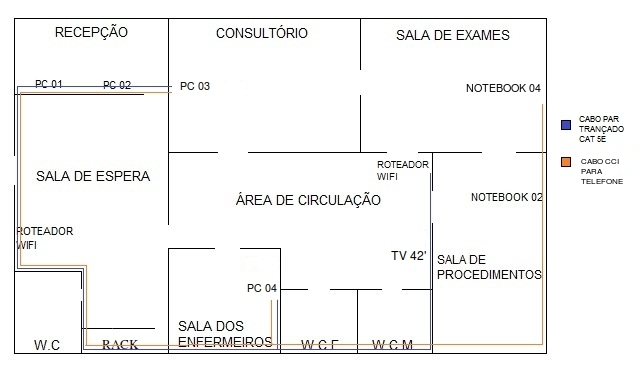
\includegraphics[width=\textwidth]{XYZ}
	\caption{Estrutura da clínica XYZ}
	\label{XYZ}
\end{figure}

\subsection{Topologia}

Foram utilizados 32 metros de cabo de rede categoria 5e para chegarmos em todos os nós da rede (computadores e roteadores, além da televisão), juntamente com 35 metros de cabo cci para a passagem de linha telefônica. Todos os cabos foram passados por um eletroduto. 

Os cabos passam horizontalmente pelos eletrodutos para chegar nos pontos necessários, fazendo o menor caminho possível visando a economia de cabos. Também todos os cabos foram devidamente crimpados. As tomadas foram bem dispostas, totalizando 7 tomadas de parede RJ45 categoria 5e e 5 tomadas de parede RJ11 categoria 3, juntamente com 7 espelhos de parede (2 tomadas por espelho).

Foram adquiridos 2 roteadores wireless 2.4ghz 1200MB para serem acoplados nas paredes para a transmissão do sinal de internet sem fio. O rack 19" 12U de parede com 3 brackets e porta frontal é composto de 1 roteador do provedor de internet, 1 switch de 16 portas 10/100/1000 mbps e 1 patch panel de 16 portas categoria 5e.


\subsection{Encaminhamento}
Os cabos serão passados pela estrutura da sala por meio de 35 metros de eletrodutos.


\subsection{Memorial descritivo}
\begin{itemize}

\item 32 metros de cabo de rede categoria 5e - 90,00 reais;

\item 35 metros de cabo cci - 92,00 reais;

\item 35 metros de eletroduto - 70,00 reais;

\item 7 tomadas de parede rj45 categoria 5e - 7,00 reais;

\item 5 tomadas de parede rj11 categoria 3 -  5,00 reais;

\item 12 ponteiras rj45 - 3,00 reais;

\item 5 ponteiras rj11 - 16,00 reais;

\item 7 espelhos de parede duplo - 105,00 reais;

\item 2 roteadores wifi 2.4ghz 1200mb 3 brackets - 460,00 reais;

\item 1 rack 19" de parede 12u com porta frontal - 400,00 reais;

\item 1 switch de 16 portas 10/100/1000 mbps - 450,00 reais;

\item 1 patch panel 16 portas cat5e - 600,00 reais;

\end{itemize} 

\subsection{Identificação dos cabos}

Os cabos de rede serão identificados no patch panel, contendo o nome do computador a qual ele está conectado.

\section{Implantação}

Será removida toda a instalação anterior que estava defasada, a realização da montagem dos eletrodutos e da passagem dos cabos será feita pela equipe de suporte e manutenção da empresa.

A equipe de T.I irá fazer a montagem do rack, assim como toda a configuração do switch, roteadores, wifi e certificações.

\section{Plano de certificação}

A certificação será realizada pela própria empresa, com os técnicos capacitados. O equipamento é anteriormente calibrado para realizar os testes com a maior precisão possível.

Depois de calibrado o equipamento, todos os cabos da rede serão testados por meio de seus passivos e do patch panel, usando como equipamento de teste o certificador Lantek 6R. Toda a bateria de teste do certificador será feita, garantido o máximo possível de estabilidade e segurança para a rede.

Os relatórios de todos os testes realizados serão entregues para o contratante, garantindo a comprovação que a rede foi corretamente instalada.

\section{Plano de manutenção}

Serão realizadas revisões periódicas anuais na rede, conforme combinado em contrato.

\subsection{Plano de expansão}

Atualmente, não existe plano de expansão para a rede. Porém, caso a empresa deseje aumentar sua capacidade, toda a estrutura já estara pronta no rack e com os eletrodutos já instalados, somente sendo necessário adicionar os novos ativos e passivos desejados.

\section{Risco}
Atualmente e com todas as certificações em dia, não existem riscos eminentes no projeto. Caso algo extraordinário aconteça, é necessário comunicar a empresa imediatamente.

\section{Orçamento}
O orçamento total dos custos de equipamento ficará em 2298 reais, mais o custo dos serviços de certificação e instalação da rede na empresa.

\section{Recomendações}
A empresa recomenda que somente usuários qualificados façam o manuseio dos equipamentos instalados, conforme foram instruídos pelos funcionários da empresa. Toda e qualquer manutenção fora do cronograma deve ser comunicada imediatamente.

\end{document}